\subsection{Loading datasets with more than 8 masses}
\setcounter{step}{0}

\goldbox{Work in progress}
During a~typical NanoSIMS measurement, at most 8~different ionic species are recorded: 7~different isotopes, and secondary electrons (normally denoted as \ttt{Esi}). This explains the visual design of LANS, which contains 8~fields for \lanstf{detected masses}. However, NanoSIMS instrument can operate in a~so-called peak-switching mode, which allows quasi-simultaneous detection of up to 15~different ionic species ($2\times 7$ different isotopes and \ttt{Esi}). This section explains how to use LANS to analyze datasets containing counts of more than 8~ionic species.
\tcbe

This feature was added to LANS based on a~request from Dr.~Gregory Stryhanyuk (UFZ Leipzig). In the example below, we use one of the datasets acquired in his lab using this approach: \ttt{2022-01-25-OPG\_1.im.zip}.

\s Load the raw dataset.

\nb\bul This can be done in the usual way, as for any other dataset. Based on the structure of the data within the binary file, LANS will automatically recognize that it was acquired in a~peak-switching mode and rearrange the data accordingly:
\begin{center}
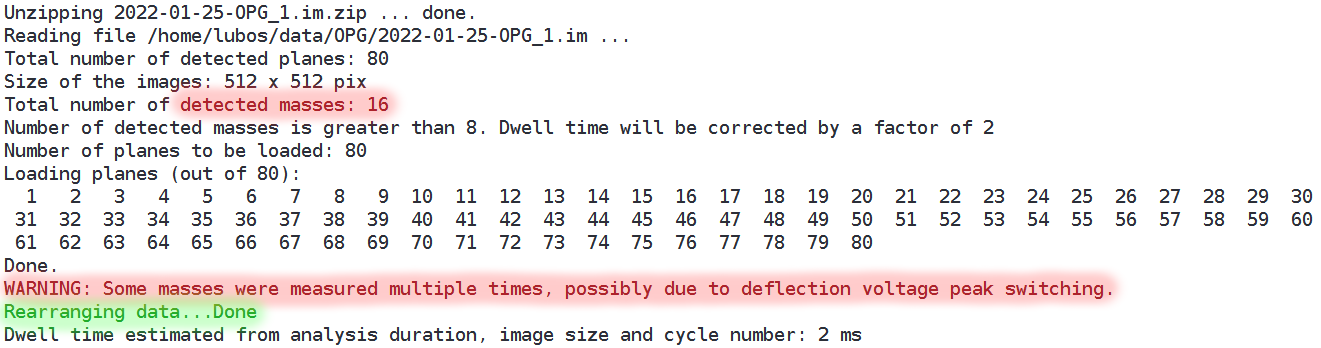
\includegraphics[scale=0.34]{figs8/LANS-8plus-load}
\end{center}

\s After loading, it is a~good idea to first find out which ions were actually detected. This is best done by selecting \lans{Input} $\ra$ \lans{Autoscale plane images}.

\nb\bul In this example, 12 different ions were detected: ${}^{16}\mathrm{O}{}^1\mathrm{H}$, ${}^{16}\mathrm{O}{}^2\mathrm{H}$, ${}^{12}\mathrm{C}_2$, ${}^{12}\mathrm{C}{}^{13}\mathrm{C}$, ${}^{12}\mathrm{C}{}^{14}\mathrm{N}$, secondary electrons (\ttt{Esi}), ${}^{12}\mathrm{C}{}^{15}\mathrm{N}$, ${}^{32}\mathrm{S}$, ${}^{12}\mathrm{C}_2{}^{1}\mathrm{H}$, ${}^{12}\mathrm{C}_2{}^{2}\mathrm{H}$, ${}^{13}\mathrm{C}{}^{14}\mathrm{N}$, and ${}^{31}\mathrm{P}{}^{1}\mathrm{H}$, as follows from the output in the Matlab console:
\begin{center}
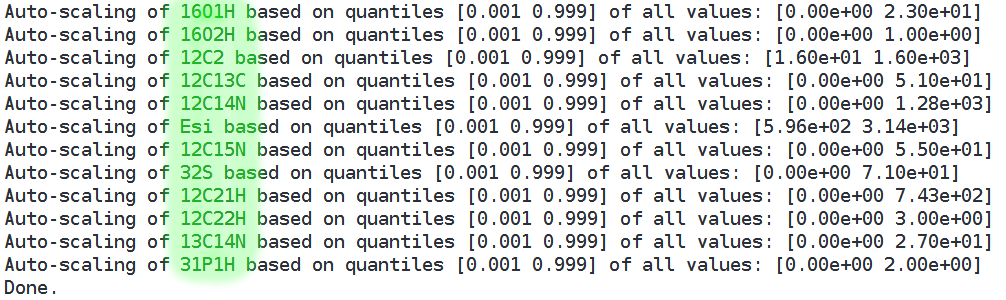
\includegraphics[scale=0.34]{figs8/LANS-8plus-autoscale}
\end{center}

\bul Due to the limit of a maximum of 8 fields in the LANS user iterface, all of these ionic species cannot included in the list of detected \lanstf{masses}. Nevertheless, they \emph{are} registered internally within the list of detected masses and can therefore be used in any of the \lanstf{expressions} (see below).

\s Select \lans{Input} $\ra$ \lans{Display images for all masses} to view the raw ion counts, plane by plane.

\begin{figure}[!ht]
\centering
\begin{tabular}{r}
A: 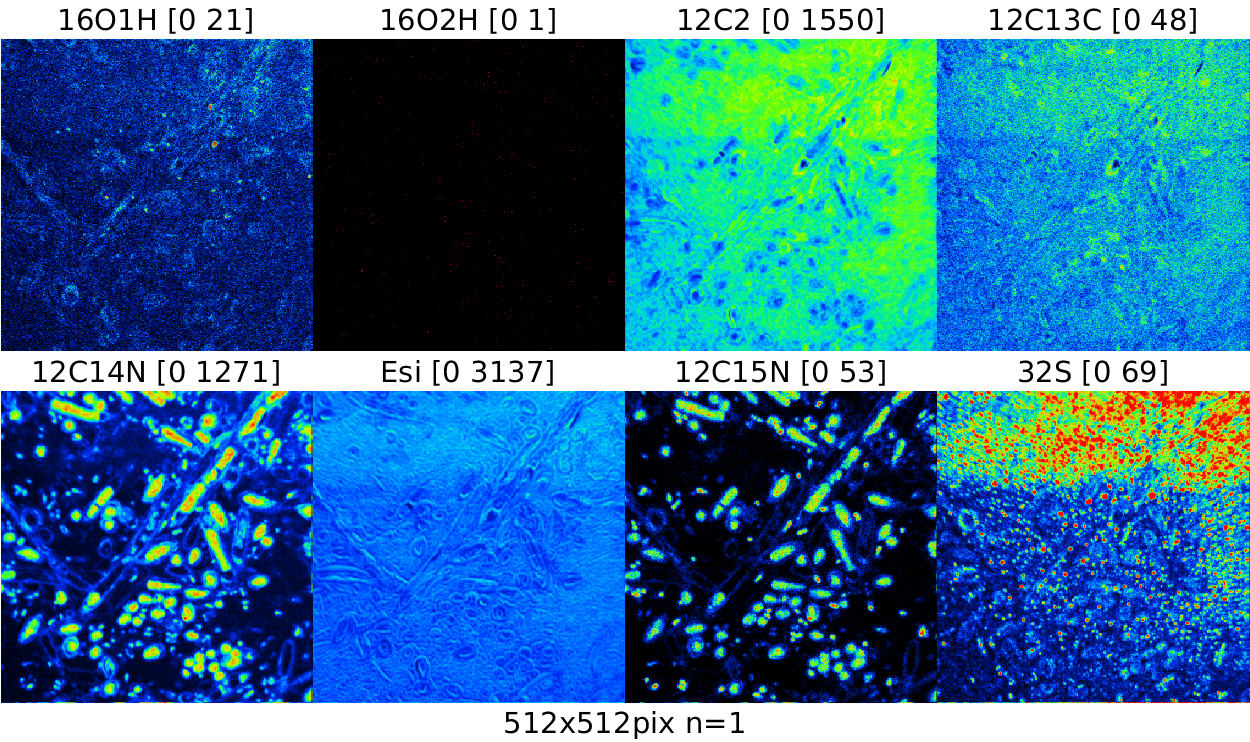
\includegraphics[scale=0.6, valign=t]{figs8/m-001}
\\
B: 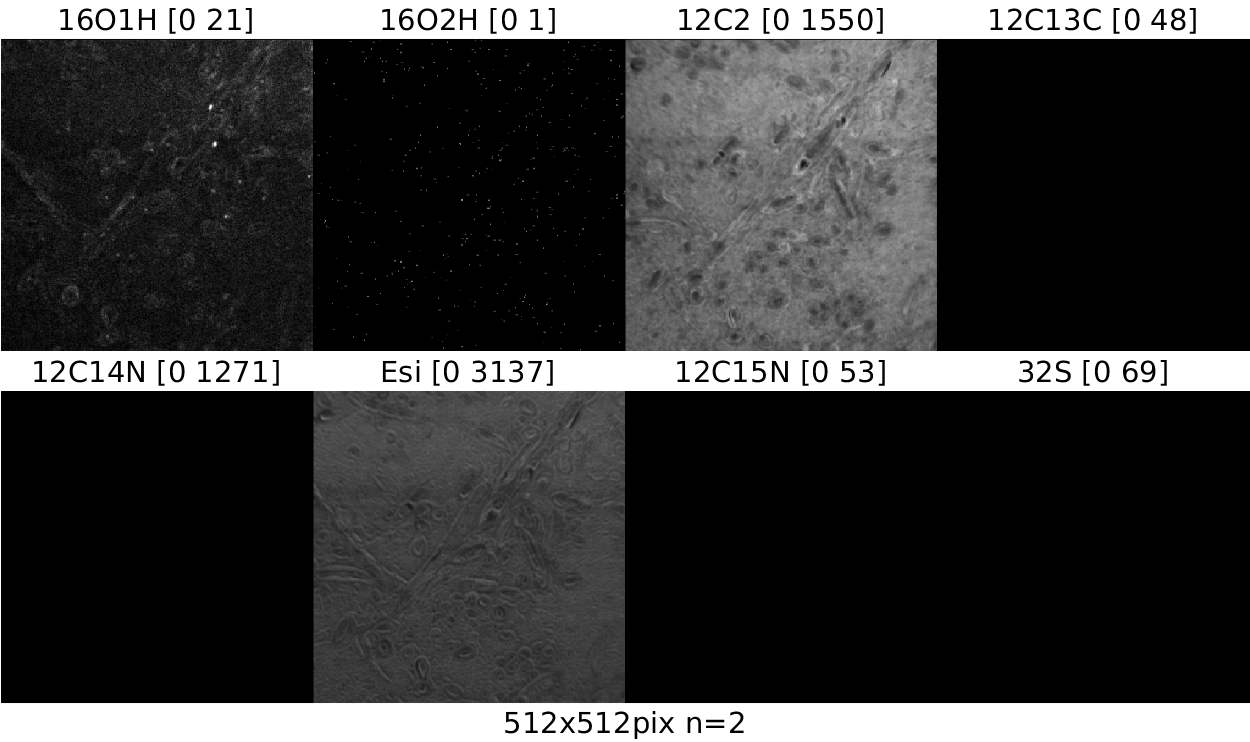
\includegraphics[scale=0.6, valign=t]{figs8/m-002}
\end{tabular}
\caption{\label{fig:LANS-8plus-frames}%
Add text.}
\end{figure}

\def\scf{0.4}
\begin{figure}[!ht]
\centering
\begin{tabular}{ccc}
A & B & C \\
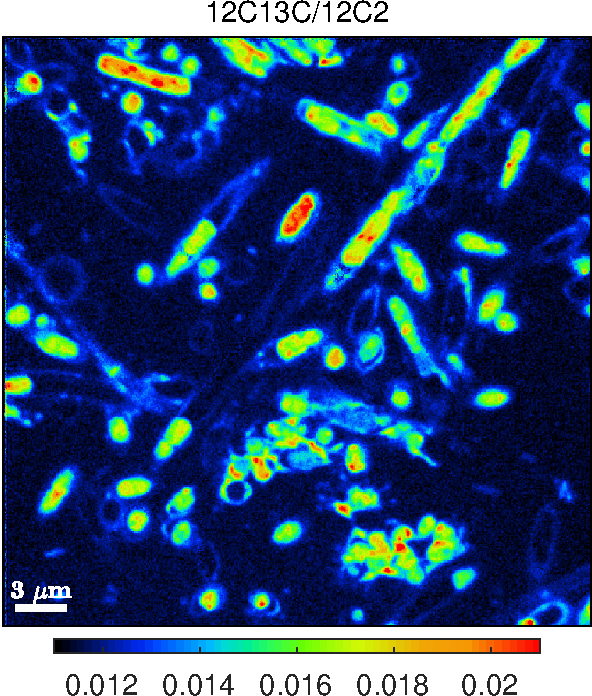
\includegraphics[scale=\scf, valign=t]{figs8/12C13C-12C2}
&
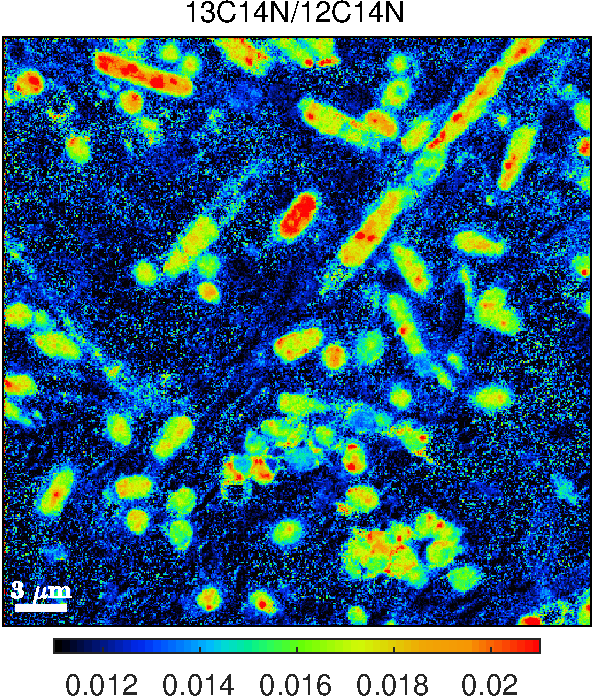
\includegraphics[scale=\scf, valign=t]{figs8/13C14N-12C14N}
&
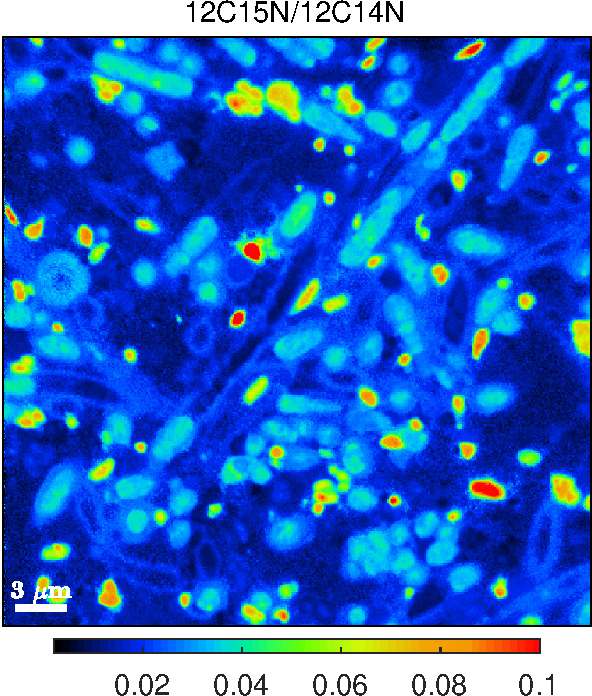
\includegraphics[scale=\scf, valign=t]{figs8/12C15N-12C14N}
\\
D & E & F\\
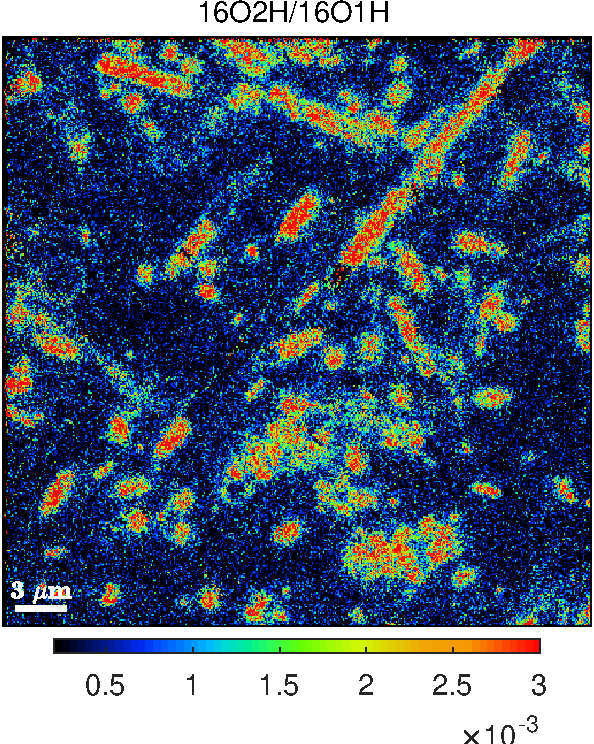
\includegraphics[scale=\scf, valign=t]{figs8/16O2H-16O1H}
&
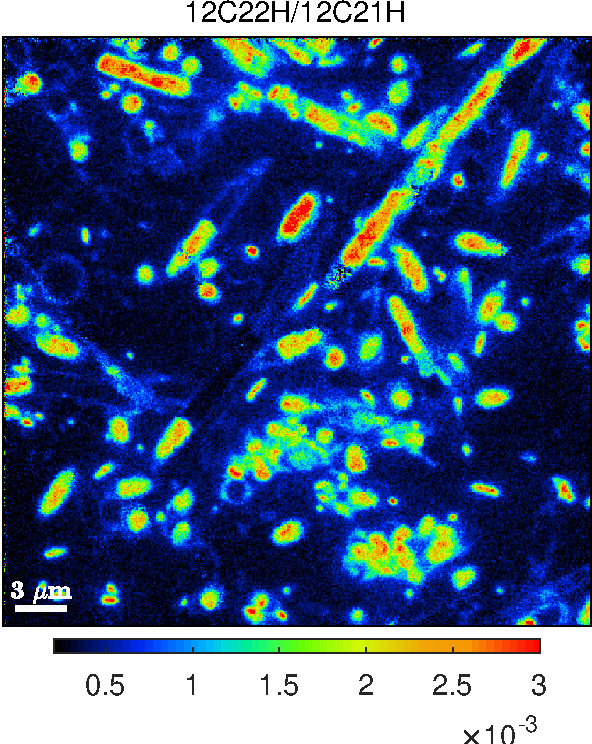
\includegraphics[scale=\scf, valign=t]{figs8/12C22H-12C21H}
&
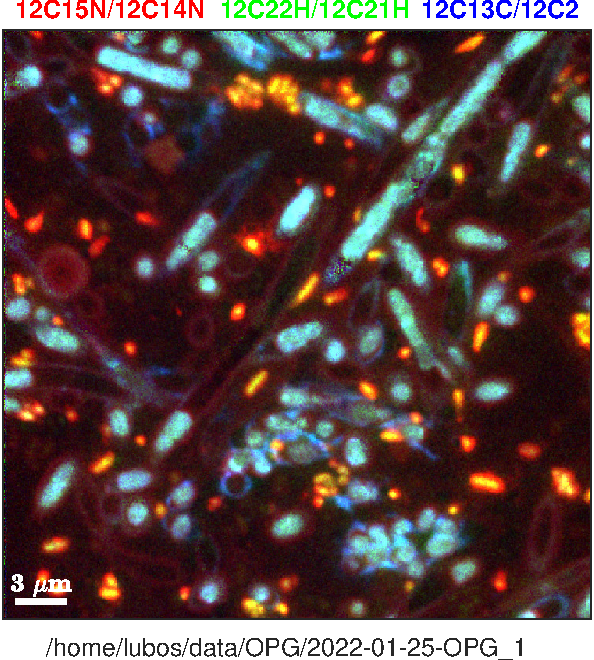
\includegraphics[scale=\scf, valign=t]{figs8/12C15N-12C14N-vs-12C22H-12C21H-vs-12C13C-12C2-rgb}
\end{tabular}
\caption{\label{fig:LANS-8plus-ratios}%
Add text.}
\end{figure}
